\documentclass[a4paper,12pt]{report} %style de document
\usepackage[utf8]{inputenc} %encodage des caractères
\usepackage[french]{babel} %paquet de langue français
\usepackage[T1]{fontenc} %encodage de la police
\usepackage[top=2cm,bottom=2cm,left=2cm,right=2cm]{geometry} %marges
\usepackage{graphicx} %'affichage des images
\usepackage{titlesec}
\usepackage{url}
\usepackage{verbatim}
\usepackage{hyperref}
\usepackage{listings}
\usepackage[linesnumbered,ruled]{algorithm2e}%linesnumbered permet de numeroter les lignes, ruled permet un affichage avec des lignes separatrices

\titleformat*{\section}{\LARGE\bfseries}
\titleformat*{\subsection}{\large\bfseries}
\def\thesection{\Alph{section}}
\def\thesubsection{\thesection.\arabic{subsection}}
\graphicspath{{images/}}

\begin{document} %début du document



%----------------------------------
%page de garde
%----------------------------------

\begin{titlepage}
	\begin{center}
		\Huge{Année universitaire 2017-2018}\\
		\Huge{Université de Caen Basse-Normandie}\\[7cm]	
		
		\Large{Rapport TPA (Lecteur de musique augmenté)}\\[2cm]
		\normalsize{ZAIZAFOUN Sami et JACQUELINE Martin}\\[0.5cm]
		\small{\textit{L2 Informatique}}
		\medskip
		\vspace{5cm}
	\end{center}
\end{titlepage}


%------------------------------
%sommaire
%------------------------------


\newpage
\tableofcontents
\newpage


\section{Choix du projet}

	Nous avons choisi ce projet car nous avons trouvé le concept de créer notre propre lecteur de musique intéressant. Durant la première séance de TPA, nous avons trouvé que l’utilisation du \textit{fxml} était plus simple et efficace pour créer l’interface graphique de notre programme. Donc nous avons repartie les taches entre nous. L’interface a été prise en œuvre par une personne et l’autre personne a pris en œuvre la manipulation de la lecture des différents fichiers medias et leur propriétés.
	
\section{Introduction}

	Le projet que nous avons sélectionné est un lecteur de musique, nous nous sommes lancés dans l'optique de faire un programme avec une interface utilisateur extrêmement claire.\\
	
	Nous souhaitions en premier lieu ajouter une recherche de parole, permettant à l'utilisateur d'avoir, dès que sont appareil est connecté à internet, un affichage simple et lisible des paroles. Le programme se devait donc de ne pas être à une taille réduite. 
	Nous avons par la suite ajouter une possible playlist alternative contenant les "favoris" à savoir les musiques jouées plus de \textit{x} fois. Nous voulions que l'application ne soit pas trop imposante, ne prenant qu'une petite partie de l'écran. 
	Nous avons donc passé quelques temps de recherche dès le début de la réflexion à chercher la taille permettant d'allier de manière optimale une bonne visibilité et lecture pour l'utilisateur et, pour autant la plus simple et petite possible.\\
	
	Nous allons ci-dessous aborder la conception en elle-même du programme.

\section{Cahier des charges}

	fonction    : lecteur de musique
	\begin{itemize}
		\item objectif    : créer la base du programme, le lecteur de musique basique et fonctionnel
		\item description : création des fonctions permettant la lecture d'une musique et d'une interface permettant de les utiliser
		\item contraintes : gérer l'interface pour qu'elle permette le futur ajout des paroles et des favoris
		\item priorité    : haute
	\end{itemize}
	\vspace{3mm}
	fonction    : ajout des paroles
	\begin{itemize}
		\item objectif    : récupérer les paroles et les afficher
		\item description : créer les fonctions permettant la récupération des paroles et son affichage 
		\item contraintes : avoir une récupération rapide, lisible (retour a la ligne, taille text, etc...)
		\item priorité    : moyenne
	\end{itemize}
	\vspace{3mm}
	fonction    : ajout des favoris
	\begin{itemize}
		\item objectif    : compter le nombre de lecture pour chaque musique et permettre l'ajout d'une musique dans les favoris
		\item description : créer les fonctions permettant le comtage du nombre de lecture de chaque musique pour l'ajouter au bout de x lancement et permettre à l'utilisateur d'ajouter et supprimer des musiques au favoris
		\item contraintes : n/a
		\item priorité    : moyenne
	\end{itemize}
	
\section{Schéma UML}

	Le \textit{fxml} est un langage de balisage d'interface utilisateur basé sur \textit{xml} créé par Oracle Corporation pour définir l'interface utilisateur d'une application JavaFX.\\
En implémentant la méthode \textit{initialize(URL location, ResourceBundle resources)} qui est appelé pour initialiser un contrôleur après que son élément racine a été complètement traité, nous pouvons manipuler toutes les fonctionnalités de notre programme et du \textit{fxml}.\\
	
	Pour manipuler un programme qui utilise du \textit{fxml}, il faut un main qui ouvre le fichier \textit{fxml} et une classe qui sert comme contrôleur, dans notre cas, la classe \textit{HomeController}.
	
	\begin{figure}[ht] 		
		\centering
  		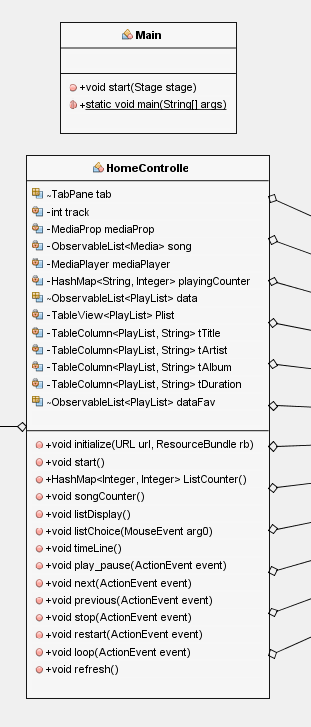
\includegraphics[scale=0.7]{Main-C} 
  		\caption{Schéma UML des classes \textit{Main} et \textit{HomeController}}
	\end{figure}
	\vspace{1cm}
	
	\newpage
	La classe \textit{HomeController} fait appel à deux classes. La classe \textit{MediaProp} et la classe \textit{PlayList}. Ces deux classes seront expliquées dans la prochaine partie.
	
	\begin{figure}[ht] 		
		\centering
  		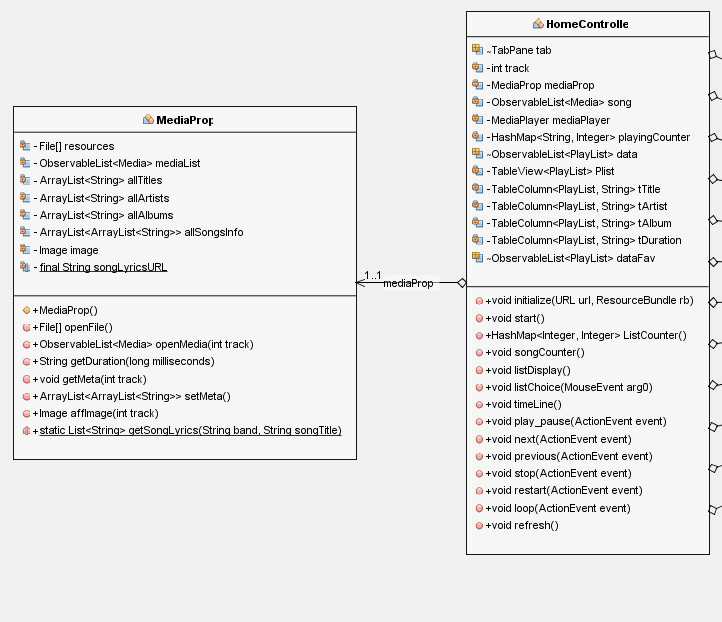
\includegraphics[scale=0.55]{C-M} 
  		\caption{Schéma UML des classes \textit{HomeController} et \textit{MediaProp}}
  		
  		\vspace{1cm}
  		
  		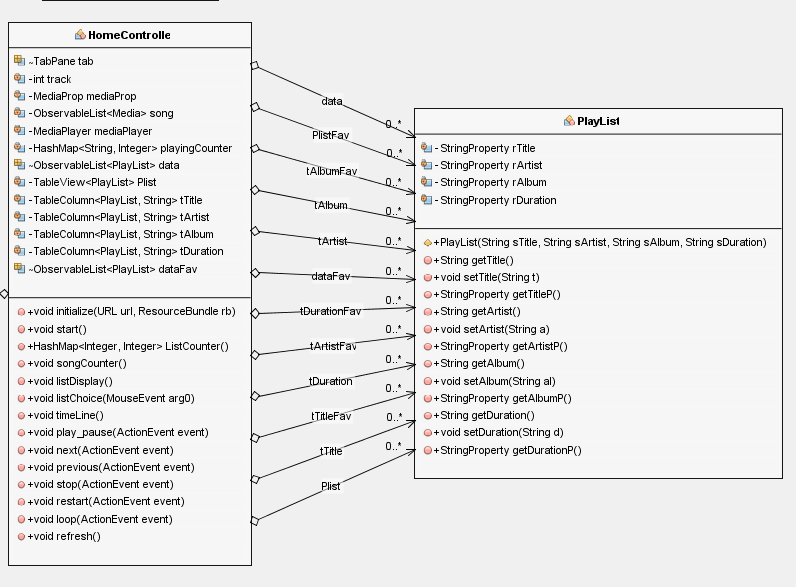
\includegraphics[scale=0.5]{C-P} 
  		\caption{Schéma UML des classes \textit{HomeController} et \textit{PlayList}}
	\end{figure}
	
\newpage
\section{Les classes}

\subsection{MediaProp}

	La classe \textit{MediaProp} sert principalement à récupérer les musiques et leurs informations. Elle récupère donc en premier temps le dossier où les médias existent en retournant une liste appelée \textit{resources} contenant tout les fichiers. Ensuite, elle récupère cette liste et elle transforme tous les fichiers en fichiers de type Media, les ajoute dans une liste puis les transforme en fichiers de type MediaPlayer, ceux-ci permettant de jouer une musique MP3.
	
	\begin{algorithm}
		\DontPrintSemicolon % Pour ne pas imprimer les ";" /!\ Certains compilateurs LaTeX demande l'utilisation de 							\DontPrintSemicolon 
		\KwIn{Integer track}
		\KwOut{List of media files}
		$mediaList \gets [ ]$\\
		$resources \gets [ \textbf{fichier musique} ]$\\
		$fichier \gets ""$\\
		\For{$f$ \textbf{in } $resources$} {
  			$fichier \gets resources[track]$\\
  			$resource \gets \textbf{path of } fichier$\\
  			$media \gets media(resource)$\\
  			$mediaPlayer \gets MediaPlayer(media)$\\
  			$mediaList+=[media,]$\\
  			$track+=1$
		}
		\Return{$mediaList$}\;
		\caption{ObservableList<Media> openMedia(int track)}
	\end{algorithm}
	
	Ensuite, nous avons une méthode qui récupère la durée de chaque musique et l'enregistre dans une variable \textit{totalTime} indépendante et variant de valeur pour chaque musique. Elle utilise alors une méthode asynchrone. Cette-dite méthode est asynchrone car elle utilise un \textit{listener} qui détecte de nouvelles informations metadata dans une musique (les metadatas étant les informations de la musique comme l'artiste, le titre, l'album, etc..). Une fois qu'une nouvelle information est détectée, la méthode cherche une clé (titre, artiste, album) et récupère sa valeur, si elle existe, puis l'insère dans une liste spécifique. Ensuite, toutes les listes sont ajoutées dans une liste \textit{allSongsInfo} qui est utilisée pour récupérer les informations quand besoin il y a. Cette liste est renvoyée dans la méthode \textit{setMeta()}.\\	
	
	De même, nous devions récupérer une photo d'album. L'idée de départ fut de récupérer les photos depuis le web mais nous fûmes confrontés au problème de tailles d'image, celles-ci différaient, certaines étant alors peu correctement présentées, et ceux malgré l'utilisation d'une méthode servant à altérer la taille des images en question. Nous avons donc récupéré les images d’album nous intéressant et nous les avons déposés dans un dossier, la méthode vérifie ensuite si le fichier MediaPlayer allant être joué possède une photo d’album associée, dans le cas contraire elle charge alors une image neutre.\\
	
	
	Pour ce qui est de la récupération des paroles, nous avons choisi d'utiliser le site web \href{http://www.songlyrics.com}{\underline{SongLyrics}}. Grâce à la librairie \textit{Jsoup.jar}, nous avons réussi à nous connecter sur ce site en utilisant le nom de l'artiste (ou du groupe les cas échéant) et le nom de la musique en remplaçant tous les espaces par des "-" et les majuscules par des minuscules (l'url du site étant généré de cette manière). Dans le cas où le programme réussi à se connecter, il récupère alors le \textit{div} contenant les paroles et l'ajoute à une liste appelée \textit{lyrics}.

\subsection{PlayList}

	La classe \textit{PlayList} permet au programme de placer les valeurs titre, artiste, album et durée dans leurs colonnes respectives du \textit{TableView} (une méthode \textit{fxml} créant un tableau). Cette classe contient principalement des méthodes dites "getter" et des méthodes "setter" qui récupèrent les valeurs et les initialisent pour en avoir l'usage ailleurs.
	
\subsection{HomeController}

	Nous allons maintenant aborder le cœur du programme, la classe \textit{HomeController} ainsi que ses méthodes.\\

	La classe \textit{HomeController} est celle qui initialise le programme car tout ce qui est en rapport avec le \textit{fxml} n'est définissable que dans cette classe. Pour bien comprendre cette classe, il faut que nous vous expliquions les fonctionnalités et les méthodes que nous avons choisi d'utiliser. \\
	
	En premier temps, la méthode \textit{listset()}. Cette méthode permet au \textit{fxml} de lier les colonnes de \textit{TableView} des musiques et des favoris avec les valeurs qui sont défini dans la classe \textit{PlayList}.\\
Une fois que ceci est fait, la méthode \textit{listDisplay()} s'occupe de l'affichage de la playlist. Pour cela, nous avons créé trois \textit{ArrayList} qui prenne les différentes listes créée dans la classe \textit{MediaProp} pour récupérer les bons titres, artistes et albums. Pour rendre ce qui est dit plus compréhensible, voici le pseudo-code:

	\begin{algorithm}
		\DontPrintSemicolon
		$meta \gets mediaProp.setMeta()$ \tcp{mediaProp.setMeta() returns a list of lists that contain a media file's information}
		$titleName \gets meta.get(0)$ \tcp{gets the title list}
		$artistName \gets meta.get(1)$ \tcp{gets the artist list}
		$albumName \gets meta.get(2)$ \tcp{gets the album list}
		\For{$i$ \textbf{in range} $file.lengeth$} {
  			$totalTime \gets song.duration$\\
  			$ele = PlayList(title, artist, album, totalTime))$ \tcp{calls the PlayList constructor while inserting the right information}
  			$data.add(ele)$ \tcp{adds the playlist into TableView}
		}
		$metaData()$ \tcp{Updates the displayed info}
		\caption{listDisplay()}
	\end{algorithm}

	Pour les favoris nous avons dû créer deux méthode : \textit{songCounter} et \textit{listCounter}. La première est exécutée dès lors qu'une musique est lancée et vérifie si le  titre de la musique qui vient d'être lancée est déjà présent dans la HashMap \textit{playingCounter}, si tel est le cas, il augmentera de un l'entier associé à ce-dit titre, dans le cas contraire il initialisera la clé du titre actuel avec la valeur 1. La seconde méthode sert, elle, a faire une HashMap proche de celle que nous venions d'aborder, ceci étant que la clé n'est plus une String qui contient le titre de la chanson mais un entier, entier qui est la valeur associé a l'entier de \textit{track} qui est le pointeur de \textit{MediaPlayer} sur \textit{File}. Cette fois ci, les musiques n'ayant pas encore été jouées voient leur valeur (associée à l'entier qui les représente) mise à 0, les autres sont au nombre de lancement incrémenté dans \textit{songCounter}. Nous obtenons donc une HashMap qui contient, dans l'ordre des fichiers, le nombre de lancement de chaque musique, nous pouvons donc très simplement retrouver quelle musique ajouter aux favoris.\\
	
	Pour rendre le programme plus facile à utiliser, nous avons créé une fonction qui permet aux utilisateurs de cliquer directement sur une musique dans la playlist pour la jouer. Cette fonctionnalité contient quelques paramètres. Un paramètre "double clique" qui permet aux utilisateurs de naviguer la playlist sans devoir commencer une musique, un paramètre qui empêche l'utilisateur d'avoir un choix nul et le paramètre qui récupère le nom de la musique et le transform en format Media pour le lancer. Ensuite, il met à jour les informations affichées et la photo de l'album.\\
Cette méthode est utilisée pour la playlist des favoris aussi.\\

	Vient ensuite, la méthode \textit{timeLine()}. Cette méthode a principalement trois fonctionnalités. 
	\begin{itemize}
  		\item Bouger la barre d'avancement avec la musique. Ceci est fait grâce à deux \textit{listener}, un qui observe la valeur de la barre et l'autre qui observe le temps passé de la musique et le premier \textit{listener} change la valeur du curseur par rapport à l'avancement de la musique.
  		\item Initialiser un minuteur qui suit l'avancement de la musique.
  		\item Un test boolean pour vérifier si l'utilisateur veut jouer la musique en boucle.
	\end{itemize}
	\vspace{5mm}	
	La classe contient aussi tout les boutons. Les fonctionnalités de ces boutons seront expliquées dans la partie \underline{\nameref{subSec:bouton}}.\\
	
	Une autre utilisation d'une barre d'avancement a été faite pour contrôler le volume dans la méthode \textit{volume()}. Le principe est plus ou moins identique à celui de la méthode d'avant. Elle utilise un \textit{listener} qui observe l'avancement du curseur et elle applique la valeur du curseur sur le volume.

\section{Manuel d'utilisation}

\subsection{Lancement}

	Le programme se lance préférablement sur \textit{Windows} de deux manière:
	
	\begin{enumerate}
   		\item Depuis un CMD en suivant les commandes:
   			\begin{figure}[ht] 		
				\centering
  				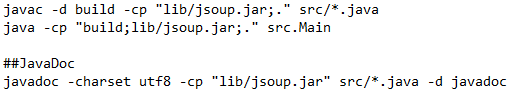
\includegraphics{exe_CMD}
			\end{figure}
			
   		\item Depuis un \textit{.bat} exécutable.
   			\begin{figure}[ht] 		
				\centering
  				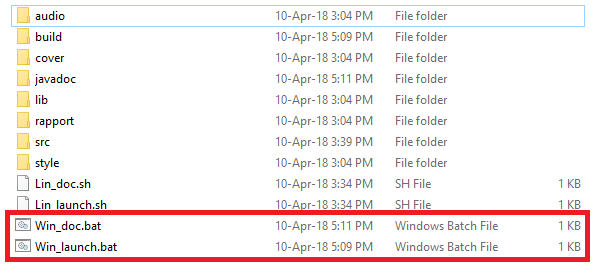
\includegraphics[scale=0.7]{bat}
			\end{figure} 
	\end{enumerate}
	
	il se lance aussi sur \textit{Linux} (sans autorisation de récupérer les paroles en ligne) de deux manière:

	\begin{enumerate}
   		\item Depuis un terminal en suivant les commandes:
   			\begin{figure}[ht] 		
				\centering
  				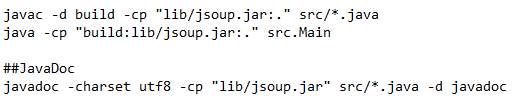
\includegraphics{exe_terminal}
			\end{figure}
			
   		\item Depuis un \textit{.sh} exécutable.
   			\begin{figure}[ht] 		
				\centering
  				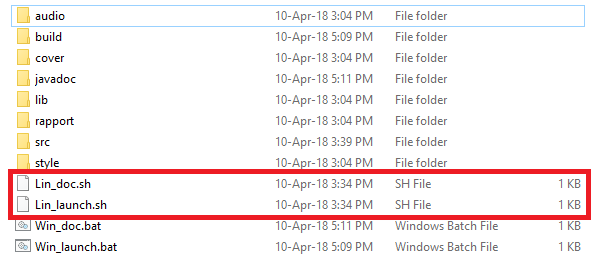
\includegraphics[scale=0.7]{sh}
			\end{figure} 
			
			En suivant les commandes: 
			\begin{figure}[ht] 		
				\centering
  				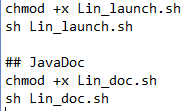
\includegraphics{Lin}
			\end{figure} 
	\end{enumerate}	
	

\newpage
\subsection{Utilisation}
	Nous avons fait en sorte que le programme soit facile à utiliser. L'interface contient trois onglets:
	
		\begin{enumerate}
   		\item L'onglet \textit{Viewer} qui affiche la musique en cours d'être jouée avec le titre, le nom de l'artiste et la photo de l'album en s'actualisant avec chaque changement de musique.
   			\begin{figure}[ht] 		
				\centering
  				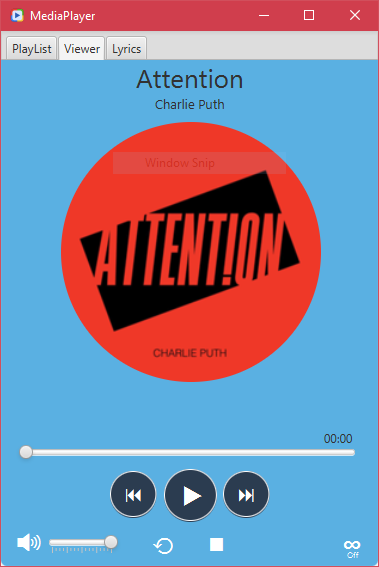
\includegraphics[scale=0.65]{overView}
  				\hspace{5mm}
  				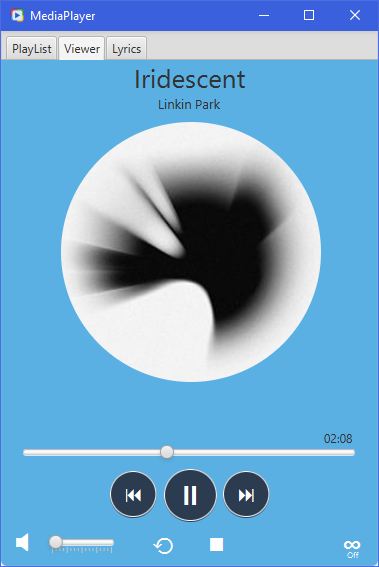
\includegraphics[scale=0.65]{overView2}
			\end{figure}
			
   		\item L'onglet \textit{Lyrics} qui affiche les paroles de la musique en cours d'être jouée.
   			\begin{figure}[ht] 		
				\centering
  				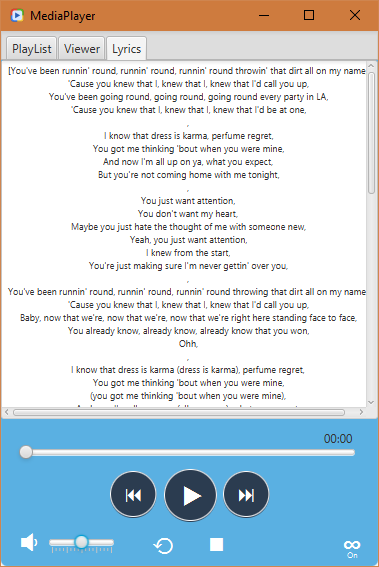
\includegraphics[scale=0.62]{lyrics}
			\end{figure} 
		
		\newpage
		\item L'onglet \textit{PlayList} qui affiche toutes les musique et la playlist des favoris.
   			\begin{figure}[ht] 		
				\centering
  				\includegraphics[scale=0.65]{playList}
  				\hspace{5mm}
  				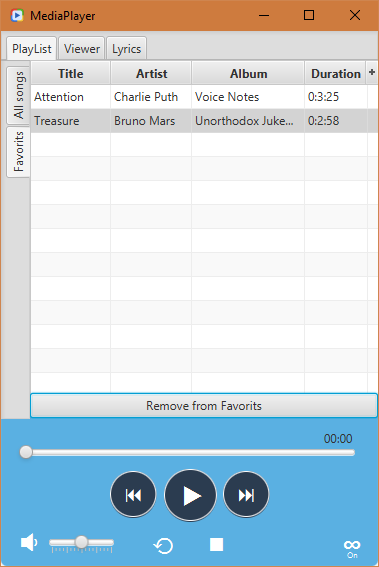
\includegraphics[scale=0.65]{favorit}
			\end{figure} 
	\end{enumerate}
	
\subsection{Les boutons} \label{subSec:bouton}

			\begin{enumerate}
   		\item Bouton Play/Pause, joue ou pause la musique en actualisant le symbol.
   			\begin{figure}[ht] 		
				\centering
  				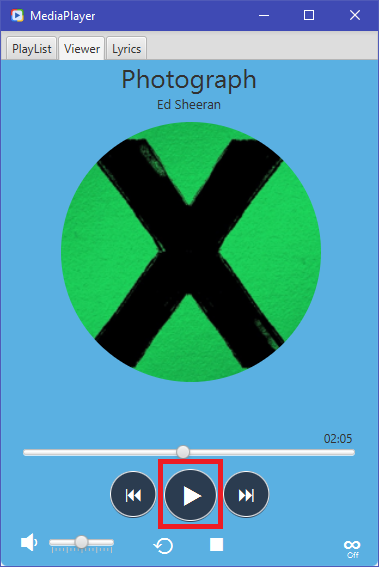
\includegraphics[scale=0.6]{play}
  				\hspace{5mm}
  				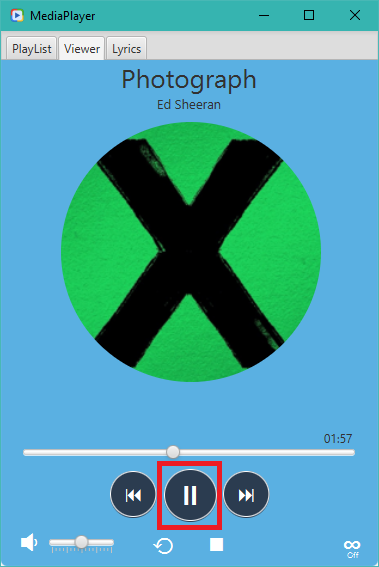
\includegraphics[scale=0.6]{pause}
			\end{figure}
		
		\newpage
   		\item Boutons Next/Previous, passe à la musique suivante ou précédente en actualisant les informations.
   			\begin{figure}[ht] 		
				\centering
  				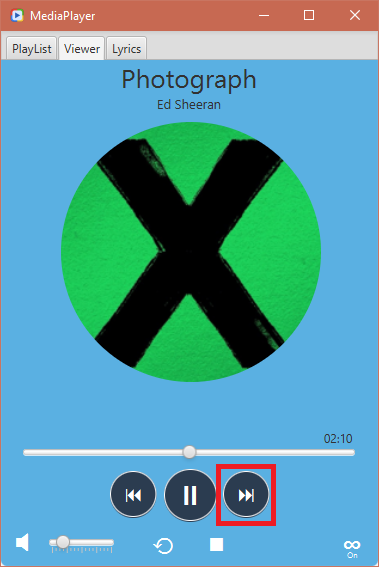
\includegraphics[scale=0.6]{next}
  				\hspace{5mm}
  				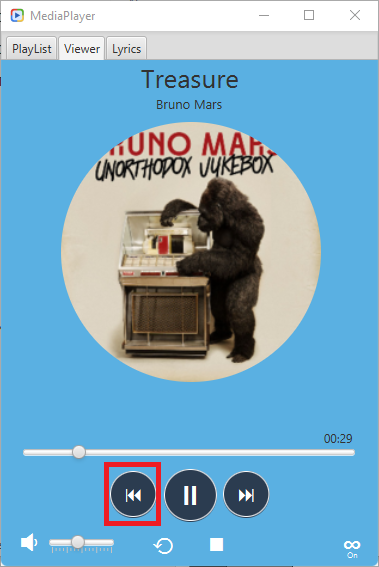
\includegraphics[scale=0.6]{prec}
			\end{figure}			 
		
		\item Boutons Restart/Stop, recommence ou arrête la musque.
   			\begin{figure}[ht] 		
				\centering
  				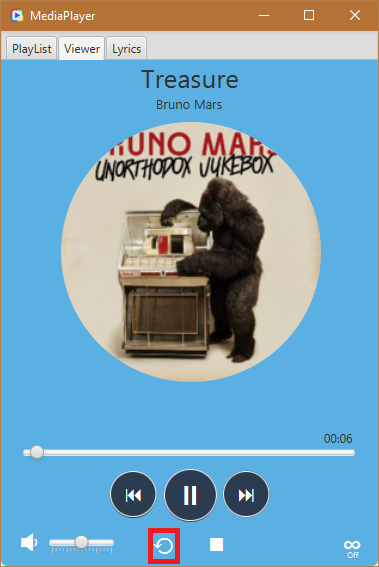
\includegraphics[scale=0.6]{restart}
  				\hspace{5mm}
  				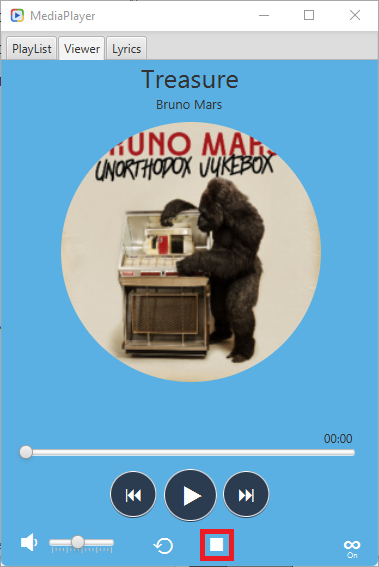
\includegraphics[scale=0.6]{stop}
			\end{figure} 
		
		\newpage
		\item Bouton Loop, met la musique en boucle.
   			\begin{figure}[ht] 		
				\centering
  				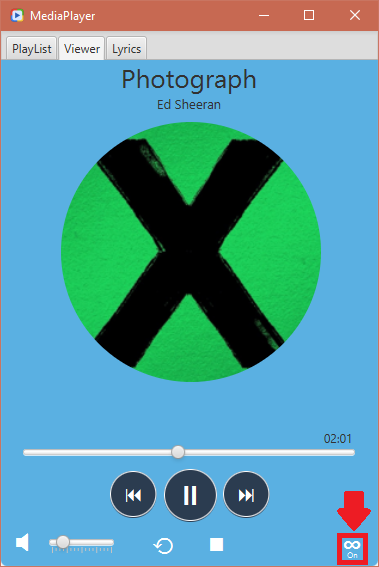
\includegraphics[scale=0.6]{loop}
			\end{figure}		
			
		\item Barre d'avancement/Volume. La barre d'avancement suit la musique en actualisant la durée passée et la barre volume modifie le son avec la possibilité de cliquer su l'icon pour muer le volume.
   			\begin{figure}[ht] 		
				\centering
  				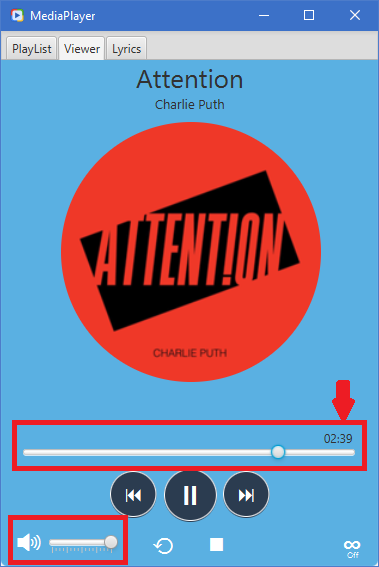
\includegraphics[scale=0.6]{slider}
  				\hspace{5mm}
  				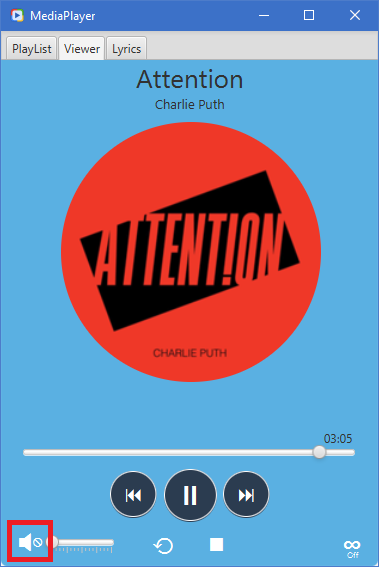
\includegraphics[scale=0.6]{mute}
			\end{figure} 
		
		\newpage
		\item Finalement, les boutons Add/Remove, permettent d'ajouter ou enlever une musique de la playlist favoris.
   			\begin{figure}[ht] 		
				\centering
  				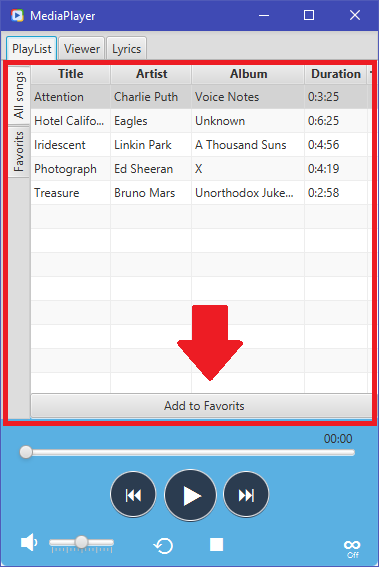
\includegraphics[scale=0.6]{add}
  				\hspace{5mm}
  				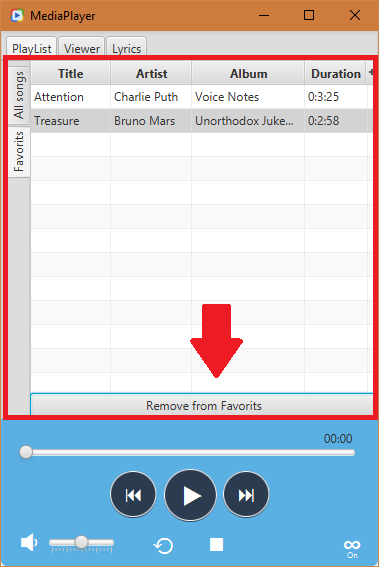
\includegraphics[scale=0.6]{remove}
			\end{figure} 
	\end{enumerate}
	
\section{Conclusion}
	Après cette description des diverses fonctions de notre programme, nous résumerons divers constats. Premièrement les améliorations possibles mais que nous n'avons pu créer du à des problèmes, que ça soit des informations difficilement trouvables, un manque de temps et une complexité de conception utilisant des choses que nous n'avons pas réussi à utiliser/comprendre.
	\begin{itemize}
		\item une visualisation animée du son en cours
		\item la création de multiples playlists
		\item la gestion de fichiers ayant d'autres extensions
	\end{itemize}
	
	Malgré cela nous avons pus nous améliorer dans bien des domaines, en voiçi quelques uns:
	\begin{itemize}
		\item l'utilisation du fxml pour une interface
		\item la gestion de fichier
		\item l'utilisation des librairies externes pour la lecture de fichier audio
		\item la gestion de fonctions asynchrones et synchrones
		\item la gestion des sliders et autres interactions avec des interfaces, que ce soit en fxml(javafx) ou en swing
	\end{itemize}
	

\newpage
\section{Bibliographie}
	La plus part de nos recherches ont été faites sur:
	
	\begin{itemize}
		\item \href{https://stackoverflow.com/}{\underline{Stack Overflow}}.
		\item \href{https://docs.oracle.com/javase/8/}{\underline{Oracle}}.
		\item Des question posées durant les heures de TP. 
	\end{itemize}
	
\section{Fin}
	
	Nous vous remercions d'avoir lu ce rapport jusqu'au bout et de vous être penché sur ce programme.\\	
	Cordialement, Mr. ZAIZAFOUN et Mr. JACQUELINE.
\end{document}